\begin{question}
\begin{center}
\measureme{\begin{tabular}{|c|c|>{\raggedright\arraybackslash}m{400pt}|}\hline
\multirow{4}{*}{\textbf{Para preguntar}}  & Cosa  & ¿Qué?   \\\cline{2-3}
  & Tiempo  & ¿Cuándo? ¿Con cuántos? / ¿Desde cuándo? / ¿Hasta cuándo?/ ¿En qué año?   \\\cline{2-3}
  & Cantidad  & ¿Cuánto/a/os/as?  \\\hline
\end{tabular}}
\end{center}

\parbox{300pt}{\raggedright 
\begin{center}
	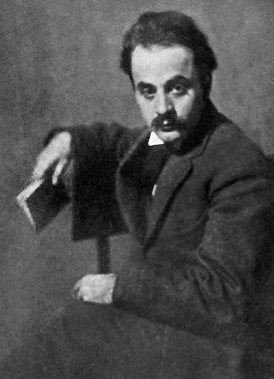
\includegraphics[width=0.2\textwidth]{NonQuestions/Figure_Slide_22.jpg}
\end{center}	
	
	}\parbox{430pt}{\raggedright \vspace*{20pt}
	
Ejemplos	

\begin{itemize}
	\item \textit{\textbf{¿Qué} es esto?}
	\item \textit{\textbf{¿Cuándo} empezó a vivir en los Estados Unidos?}
	\item \textit{\textbf{¿Con cuántos} años murió?}
	\item \textit{\textbf{¿En qué} año nació Khalil Gibran?}
\end{itemize}	
	}\vspace*{20pt}	
	
La partícula “cuánto” concuerda con el nombre que sigue.
	
\end{question}